\documentclass[Main]{subfiles}
\begin{document}


\chapter{System architectural design}
\section{System functional design}
This section describes the functional design and architecture of the system.
This is also illustrated in Figure \ref{fig:FFD} below.

\begin{figure}[H]
\centering
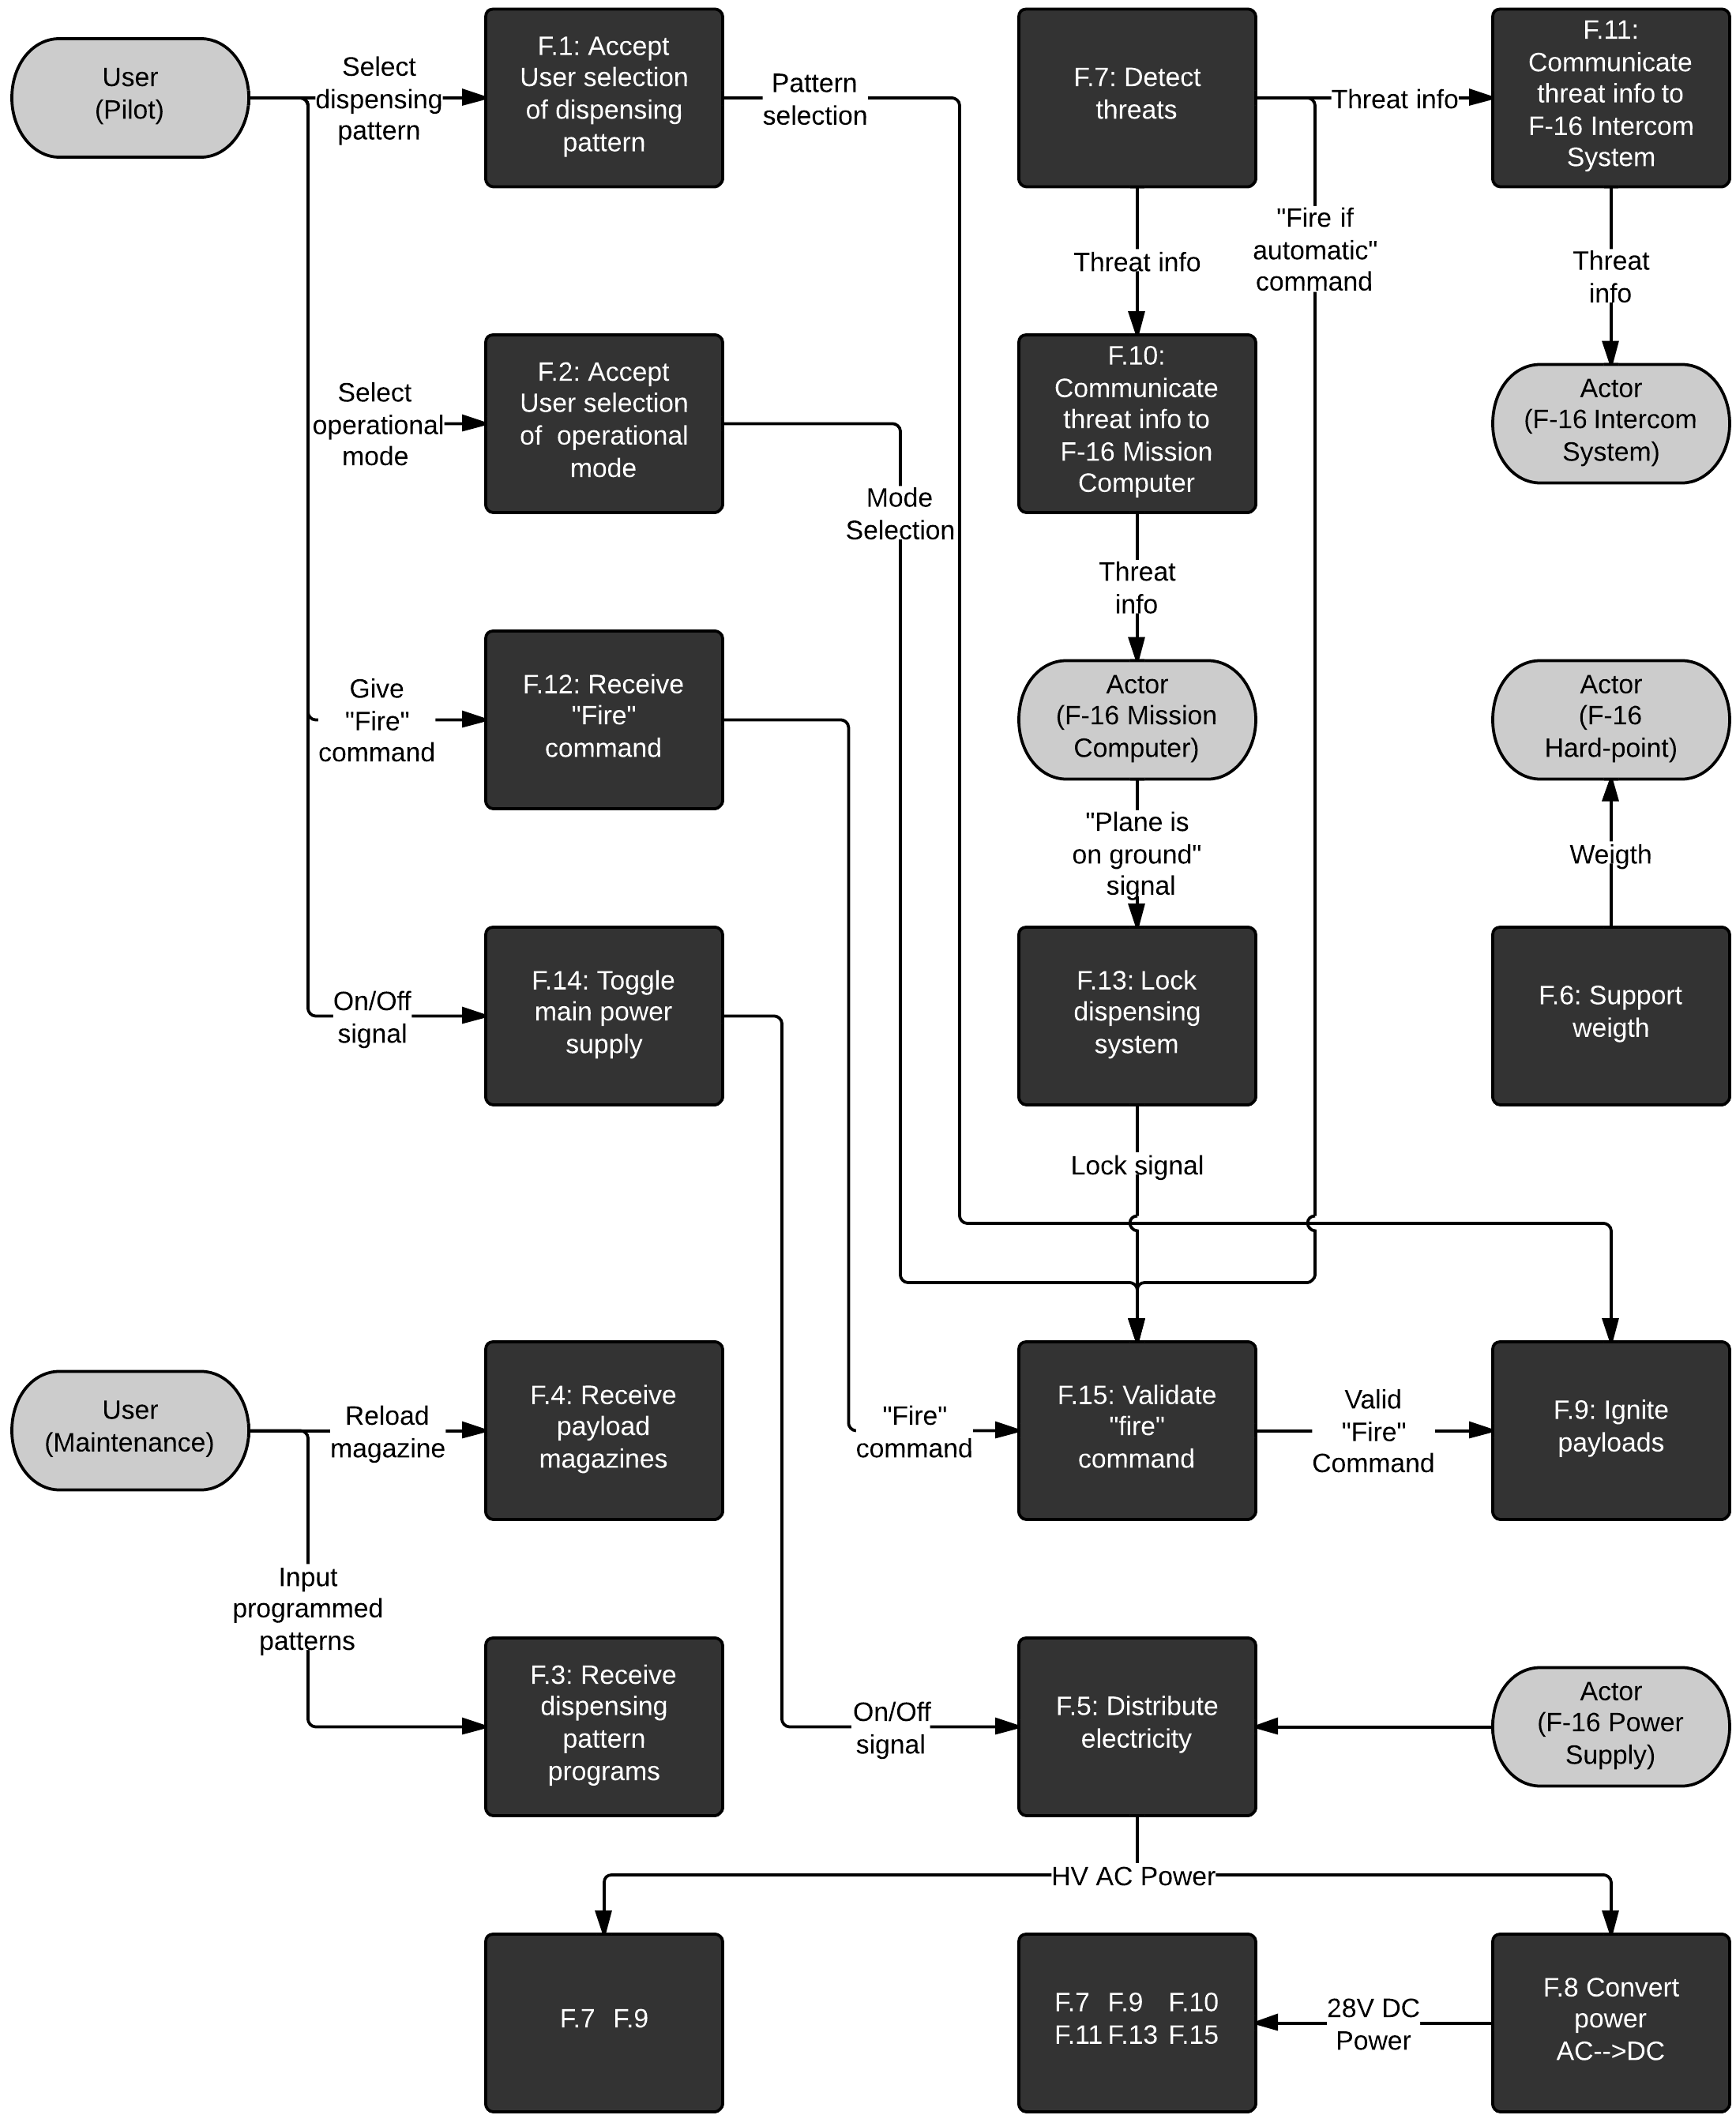
\includegraphics[width=0.80\textwidth]{FunctionalFlowDiagram}
\caption{Functional Flow Diagram}
\label{fig:FFD}
\end{figure}

\subsection{System functions}
\begin{enumerate}[label=F.\arabic*]
\item Accept User selection of dispensing pattern

Accepts dispensing pattern selection from the User in the form of a physical switch input, and outputs it to \ref{enum:Ignite}.

\item Accept User selection of operational mode

Accepts operational mode selection from the User in the form of a physical switch input, and outputs it to \ref{enum:Val}.

\item Receive dispensing pattern programs

Receives and saves predetermined chaff/flare dispensing programs

\item Receive payload magazines

Receives and stores payload magazines, ready for use

\item Distribute electricity

Distributes HV AC Power from the F-16 Power Supply and distributes it the all functions that require it (F.7-9)

\item Support weight

Distributes the weight of system to the suspension structure and the F-16 hard-point

\item Detect threats

Scans surroundings for incoming threats and alerts F.10-11. It also commands \ref{enum:Val} to fire in case of automatic operation mode.

\item Convert power AC/DC

Converts high voltage AC power from the F-16 Power Supply to 28V DC power and distributes it to the function that require it (F.7,9-11,13,15)

\item Ignite payloads\label{enum:Ignite}
\item Communicate threat info to F-16 Mission Computer
\item Communicate threat info to F-16 Intercom System
\item Receive "Fire" command
\item Lock dispensing system
\item Toggle pod power supply
\item Validate "fire" command\label{enum:Val}




\end{enumerate}


In Figure \ref{fig:ComponentsAndInterfaces} an overview of the the complete systems components and interfaces is shown. Each component and interface will described and linked with system requirements in the following sections.

\begin{figure}[H]
\centering
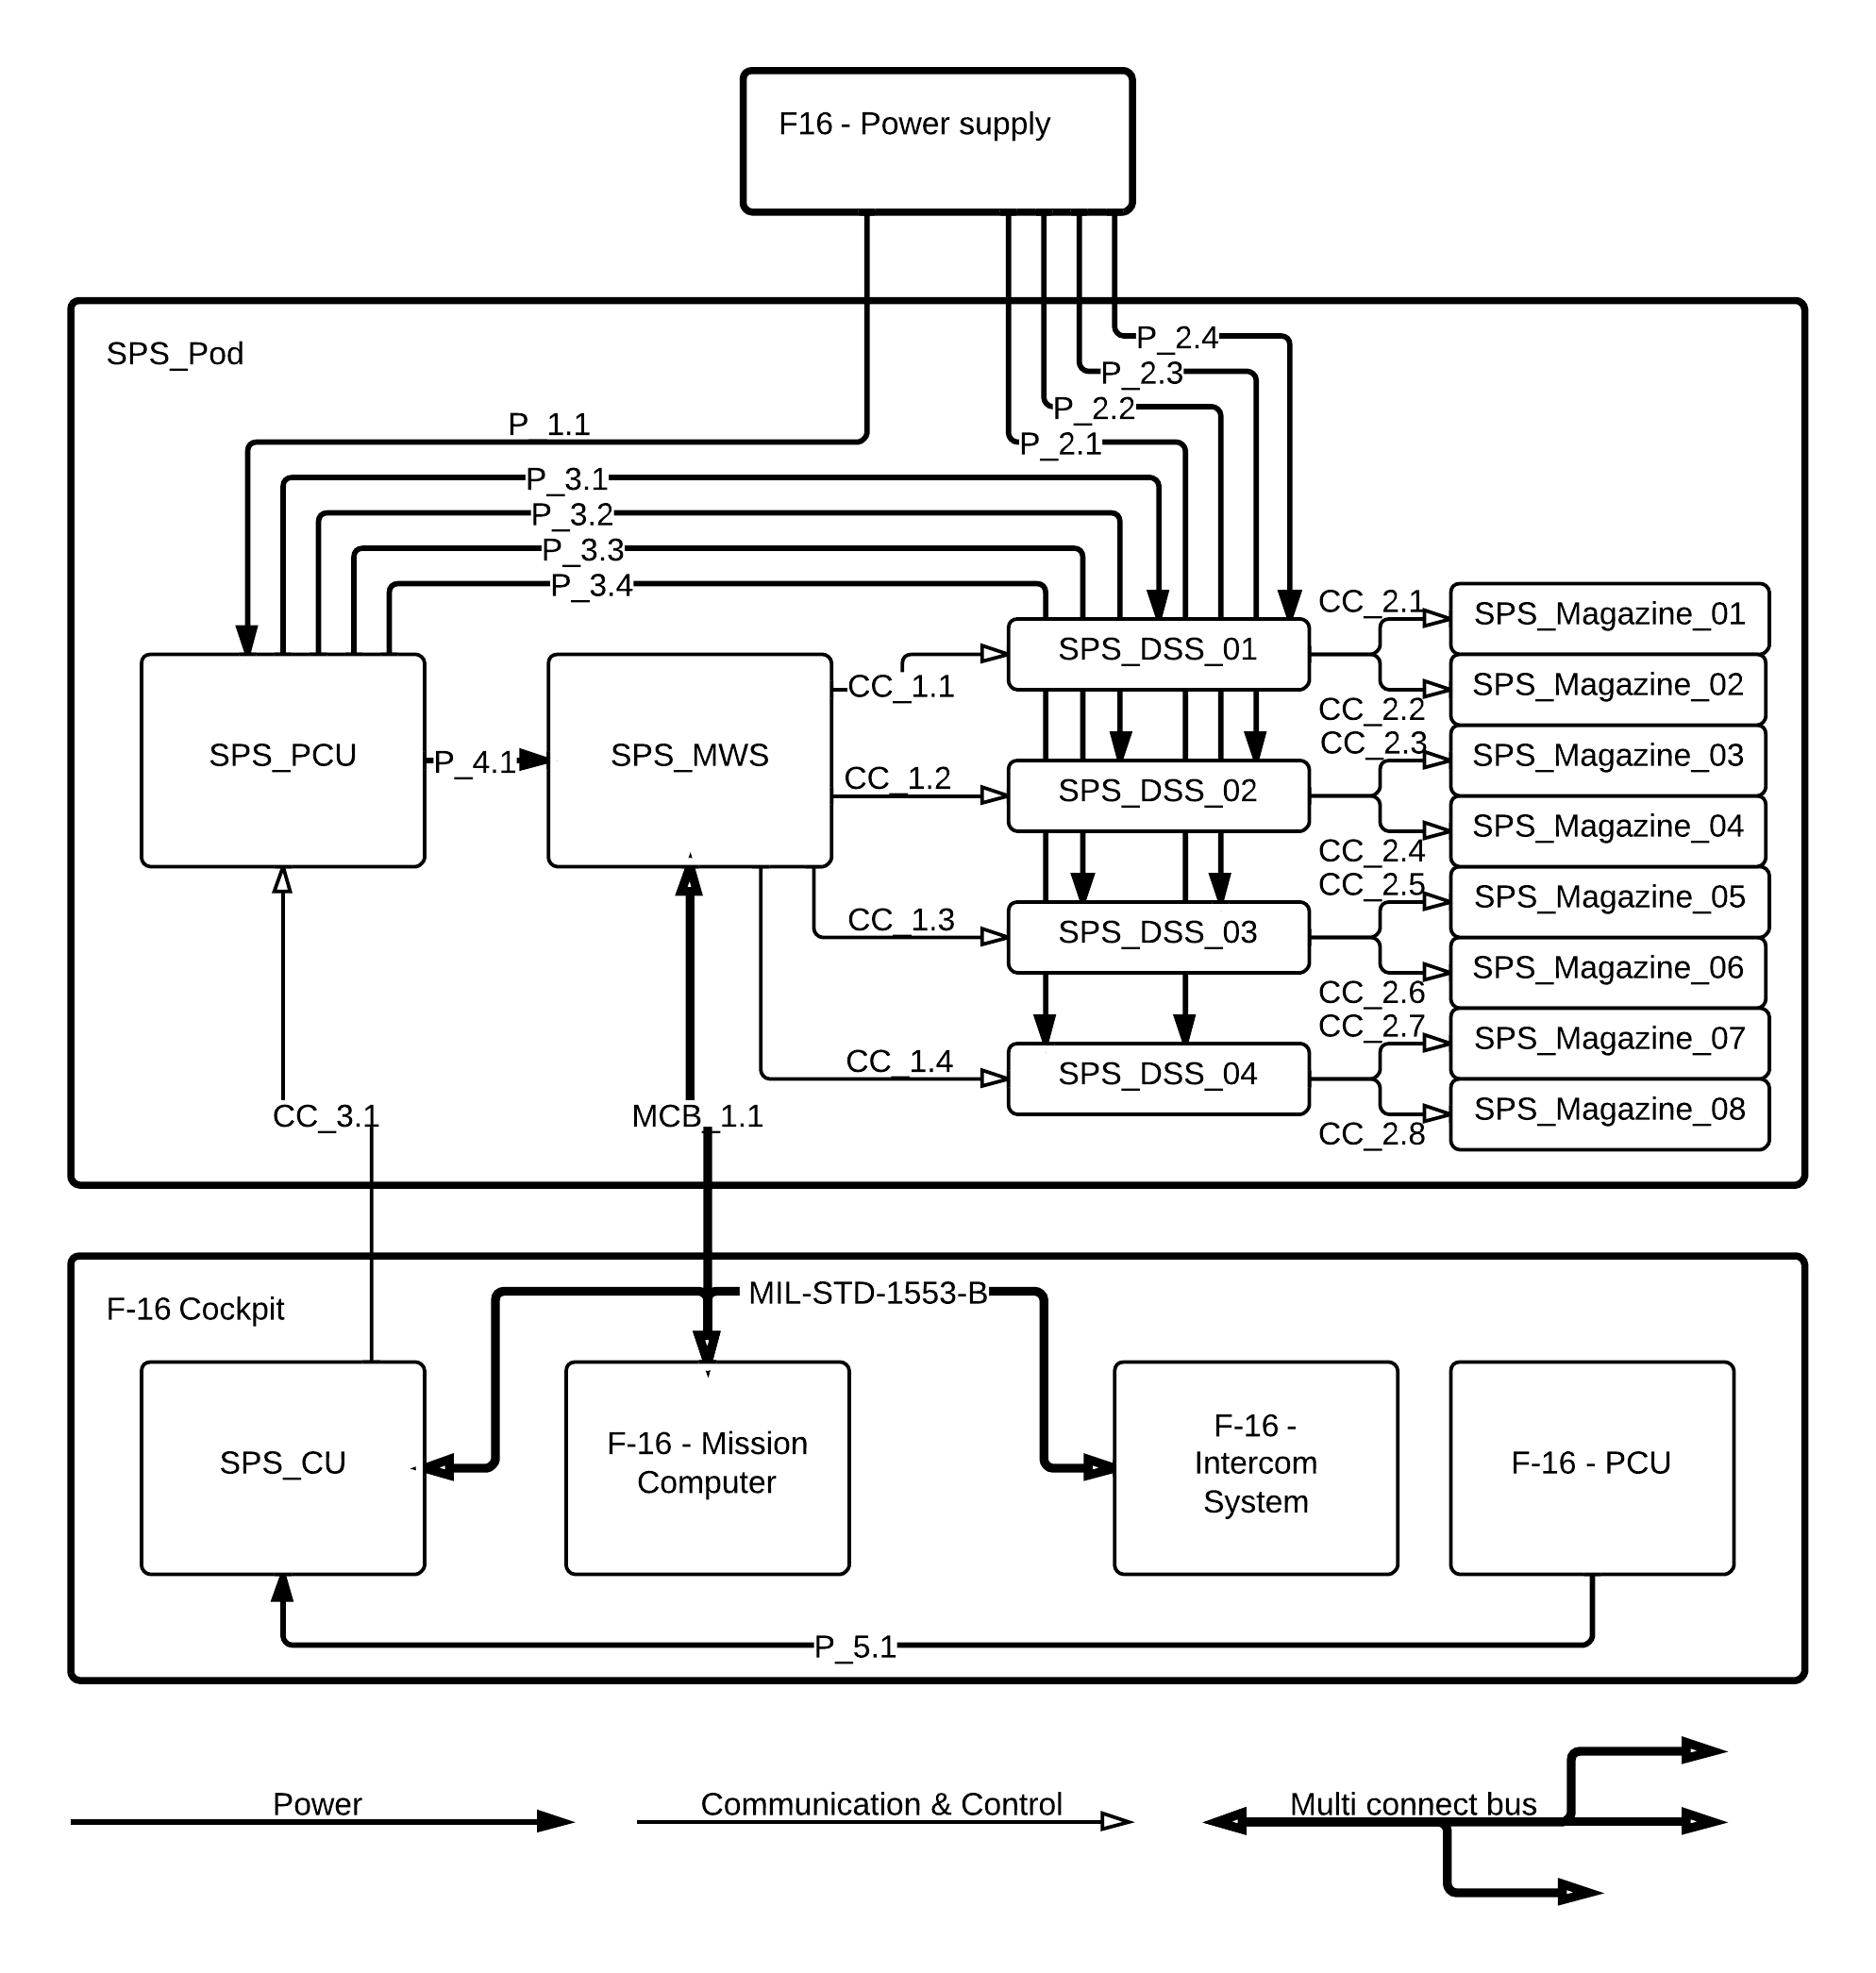
\includegraphics[width = 0.9\textwidth]{ComponentsAndInterfaces}
\caption{Components and interfaces}
\label{fig:ComponentsAndInterfaces}
\end{figure}

\subfile{SystemComponents}
\newpage
\subfile{ConceptOfExecution}
\newpage
\subfile{InterfaceDesign}
\end{document}
